\documentclass[final]{beamer}
\mode<presentation>
{
  \usetheme{PosterCERG}
}
% size in width and height is in cm
% Arch D: 24"x36" use 60.96 x 91.44 Typical size for our printer, use 3 columns, scale=0.8 to fit more text
% each column should be 0.3\linewidth
% Arch E: 36"x48" use 91.44 x 121.92 OK for FedexKinko, use 4 columns
% each column should be 0.22\linewidth
\usepackage[orientation=portrait,size=custom,width=76.2,height=106.68,scale=1]{beamerposter}
% DATE-2015 Poster format
% DIN-A0-Portrait ----1189mm X 841mm or 118.9cm x 84.1cm or 46.8in x 33.1in 
%\usepackage[orientation=portrait, size=custom, width=84.1, height=118.9 scale=1.0]{beamerposter}sd
\usepackage{multirow,wrapfig}
\usepackage[labelformat=empty,justification=centering]{caption}
\usepackage{tikz}
\usepackage{lmodern}
\usepackage{multirow}
\usepackage{listings}
\usetikzlibrary{fit,arrows,calc,positioning}
%\usepackage{wrapfig}
%%%%%%%%%%% Additional packages-Panci
\usepackage[T1]{fontenc}

\definecolor{ocean}{RGB}{0,205,255}
\definecolor{beamerbackground}{rgb}{0.5,0.5,0.3}
\newcommand{\rb}[1]{\raisebox{1.3ex}[-1.3ex]{#1}}

\newcommand{\urlwofont}[1] { \urlstyle{same}\url{#1} }
     
\graphicspath{{figures/}}
\title{\LARGE Flexible, Opensource workBench fOr Side-channel analysis\\ \vspace{0.5ex}(FOBOS)}
\author{Rajesh Velegalati, Panasayya Yalla, Jens-Peter Kaps}%\vspace{-2ex}
\institute{\vspace{-1ex}Department of Electrical and Computer Engineering, George Mason University, Fairfax, Virginia 22030, USA
           %\{pyalla, ehomsiri, jkaps\}@gmu.edu \url{http://cryptography.gmu.edu}
          } %this should be GMU etc. 
\date{March}

\begin{document}
\lstset{%
  basicstyle=\ttfamily,
  language=bash,
  commentstyle=\color{tabutter},
  keywordstyle=\color{black},
  numberstyle=\color{cergbg1},
  stringstyle=\color{ta3orange},
  identifierstyle=\color{cergbg1}
}
\begin{frame}[fragile]{} 
  \begin{columns}[t]
% ---------------------------------------------------------------------------
%   FIRST COLUMN
% ---------------------------------------------------------------------------
    \begin{column}{.31\linewidth}

% ---------------------------------------------------------------------------
      \begin{block}{Abstract}
Side-channel analysis (SCA) attacks pose a growing threat to implementations of cryptographic 
algorithms implemented in software as well as in hardware. Current standard 
side-channel evaluation boards with Field Programmable Gate Arrays (FPGAs), that allow 
for exploring the vulnerability of cryptographic implementations on FPGAs, are expensive
and available only for a few FPGA devices. Furthermore, a complete open source 
software package that includes drivers that run test cases on the board, 
control the measurement equipment, and contain several side-channel analysis 
techniques is not readily available. Each user has to assemble their own setup
based on software packages from multiple sources, written in multiple languages
and write parts themselves. Additionally, this complexity and cost makes it very difficult,
if not impossible, to educate students on side-channel analysis
through hands-on laboratory exercises. 
FOBOS is an open-source framework for conducting side-channel attacks on FPGAs
which supports multiple FPGA devices and includes all necessary software to run 
differential power analysis attacks, which are the most prominent kind of side-channel attacks. 
Through its completeness and support for educational FPGA boards it is an ideal 
teaching tool.
      \end{block}
	 
%---------------------------------------------------------------------------------

      \begin{block}{Side Channel Analysis (SCA)}
        \begin{itemize}
          \item {\color{red}Danger:} Implementations are susceptible to Side Channel Analysis (SCA).
        \end{itemize}

        \vspace{-2ex}
        \begin{minipage}[t]{0.62\linewidth}
          %\vspace{-5cm}%\small
          \begin{itemize}
            \item Key~space~256-bit,~$2^{256} = 1.2 \cdot 10^{77}$keys
            \item Atoms in Universe {\tiny(wikipedia)} $9.4 \cdot 10^{79}$
            \item SCA allows to attack 8-bit at a time
            \item SCA complexity $\frac{256}{8} \cdot 2^{8} = 8192$
          \end{itemize}
        \end{minipage}%
        %\hspace{-0.5cm}
        \begin{minipage}[t]{0.38\linewidth}  
          \vspace{-1ex}%
          \hspace{-1ex}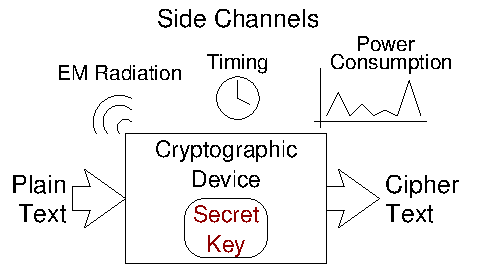
\includegraphics[width=\linewidth]{../figures/sidechannel2}
        \end{minipage}
        
        \begin{center}
        \begin{minipage}[t]{0.9\linewidth}  
        \setbeamercolor{padding}{fg=white, bg=cergbg1}
        \begin{beamercolorbox}[rounded=true]{padding}
          %\begin{block}{Danger}
          %\small%
          \begin{itemize}
            \item These are passive, non invasive attacks.
            \item They are difficult to detect.
            \item The measurement setup is not very expensive.
            \item Applies to Software as well as Hardware implementations.
          \end{itemize}
          %\end{block}
        \end{beamercolorbox}
        \end{minipage}
        \end{center}
      \end{block}
%-----------------------------------------------------------------------------------
      \begin{block}{Current SCA Evaluation Solutions}
        \begin{minipage}[t]{0.49\linewidth}
          {\large\textbf{AES}}%\vspace{1ex}
          \begin{itemize}
            \item NIST standard for block ciphers.
             \item Based on Rijndael block cipher.
            %\item Traditional block cipher.
            \item 128-bit block size.
            \item 128/192/256-bit key size.
          \end{itemize}
        \end{minipage}%
        \begin{minipage}[t]{0.49\linewidth}  
          {\large\textbf{Keccak-$p$[1600,$n_r$]}}%\vspace{1ex} %permutation
          \begin{itemize}
            \item Permutation based on Keccak, winner of competition for next Secure Hash Algorithm (SHA-3).
            \item 1600-bit state size.
            %\item Keccak is based on Sponge construction.
          \end{itemize}
        \end{minipage}
      \end{block}
%------------------------------------------------------------------------------------
          \begin{block}{Drawbacks of Current Solutions}   
            \begin{itemize}
              \item IA Meter only performs acquisition using Python.
              \item OpenSCA Toolbox performs only analysis using Matlab.
              \item SASEBO has very limited FPGA support und uses C\#.
              \begin{itemize}
                \item DPA resistance depends on FPGA family.
                \item DPA resistance depends on FPGA packaging (e.g., w/ or w/o capacitances).
              \end{itemize}
              \item Currently only a patchwork of scripts and tools exist.
              \item No complete, free, and open-source solution is available.
              \item No inexpensive out-of-the-box solution for education.
            \end{itemize}
          \end{block}
        
%---------------------------------------------------------------------------------
      \begin{block}{Modes of Operation Summary}
        \begin{table}[t]\setlength{\tabcolsep}{2.0pt}
         \centering
          \vspace{-2ex}%\large
          %\footnotesize
          \caption{AES / Rijndael* and Keccak Modes \small (Rd. = Number of rounds)}\label{tab:aesmodes}
          \begin{tabular}{|l|l|l|llll|l|l|}\hline
            &Operation  &  Mode         & Block & Key & Rd.    &\hspace{1ex}$\rho$& Inputs                    & Outputs \\ \hline
            \parbox[t]{9mm}{\multirow{6}{*}{\rotatebox[]{90}{\textbf{AES}}}}
            &Hash*      &  AES-Hash     & 256   & N/A & 14     &      &  $|M|$, $M$             & $H$       \\
            &MAC        &  CMAC         & 128   & 128 & 10     &      &  $|M|$, $M$, $K$, $IV$  & $T$       \\
            &AEAD       &  GCM          & 128   & 128 & 10     &      &  $|M|$, $M$, $K$, $IV$, & $T$, $C$  \\
            &           &               &       &     &        &      &  $|AD|$, $AD$           &           \\
            &PRNG       &  Fortuna      & 128   & N/A & 14     &      &  $S$                    & $R$       \\ \hline
            \parbox[t]{9mm}{\multirow{6}{*}{\rotatebox[]{90}{\textbf{Keccak}}}}
            &Hash       & Sponge        & 1600  & N/A & 24     & 1088 &  $|M|$, $M$             & $H$      \\
            &MAC        & Sponge        & 1600  & 128 & 24     & 1088 &  $|M|$, $M$, $K$, $IV$  & $T$      \\
            &AEAD       & Duplex        & 1600  & 128 & 12     & 1344 &  $|M|$, $M$, $K$, $IV$, & $T$, $C$ \\
            &           &               &       &     &        &      &  $|AD|$, $AD$           &          \\
            &PRNG       & Duplex        & 1600  & N/A & 12     & 1344 &  $S$                    & $R$      \\ \hline
          \end{tabular}
        \end{table}
        \hspace{1ex}
        {
          \footnotesize $M$--Message, $K$--Key, $AD$--Associated Data, $S$--Seed, $IV$--Initialization Value, 
                        $H$--Hash, $T$--Tag, \\ \hspace{3.5ex}$C$--Cipher-text, $R$--Random Number, $|X|$--Length of $X$
        }
        \\
       \end{block}

%---------------------------------------------------------------------------------
    \end{column}
% ---------------------------------------------------------------------------
%   SECOND COLUMN
% ---------------------------------------------------------------------------
    \begin{column}{.31\linewidth}
   
% ---------------------------------------------------------------------------
      
% ---------------------------------------------------------------------------
      \begin{block}{FOBOS}
        {\color{red}F}lexible {\color{red}O}pen-source work{\color{red}B}ench 
        f{\color{red}O}r {\color{red}S}ide-channel analysis, 
          loosely named after the Greek god Phobos ($\phi \acute{o} \beta o \varsigma$) is 
          an open-source framework for DPA with the following goals: 
        \begin{itemize}
          \item Complete solution useful for education.
          \item De-couples Control from Device under Test (DUT).
          \item Allows use of inexpensive FPGA boards.
          \item Modular software, allows for easy adaptation for new boards, oscilloscopes.
          \item Extensible by the user to include
          \begin{itemize}
            \item new attack scenarios and
            \item new attack models. 
          \end{itemize}
        \end{itemize}
      \end{block}
% ---------------------------------------------------------------------------
      \begin{block}{Top Level Diagram}
        \begin{center}
          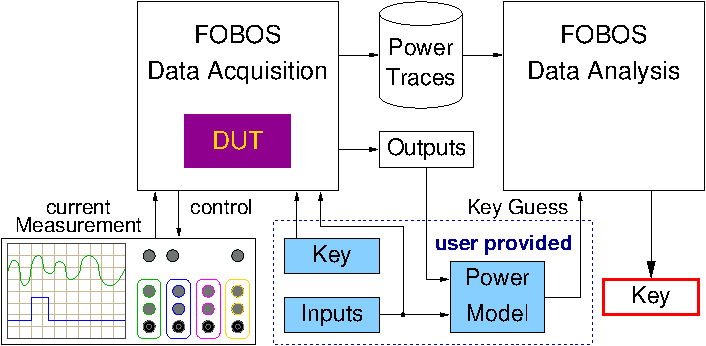
\includegraphics[scale=1.5]{../figures/fobos-top}
        \end{center} 
       \end{block}
     
% ---------------------------------------------------------------------------
      \begin{block}{FOBOS Acquisition}
        \begin{center}
          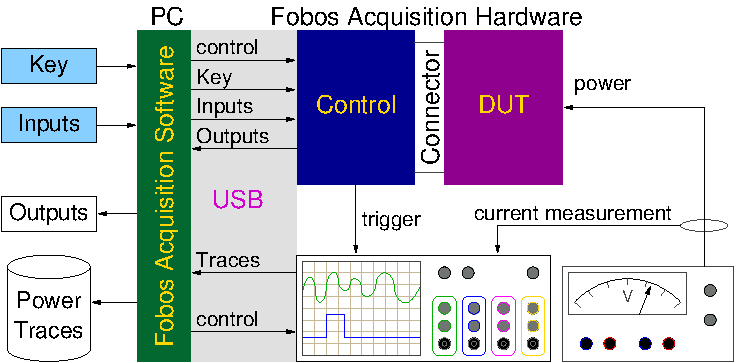
\includegraphics[scale=1.5]{../figures/fobos-dac}
        \end{center} 
       \end{block}
     
% ---------------------------------------------------------------------------
      \begin{block}{FOBOS Hardware}
        \vspace{-2ex}
        \begin{center}
          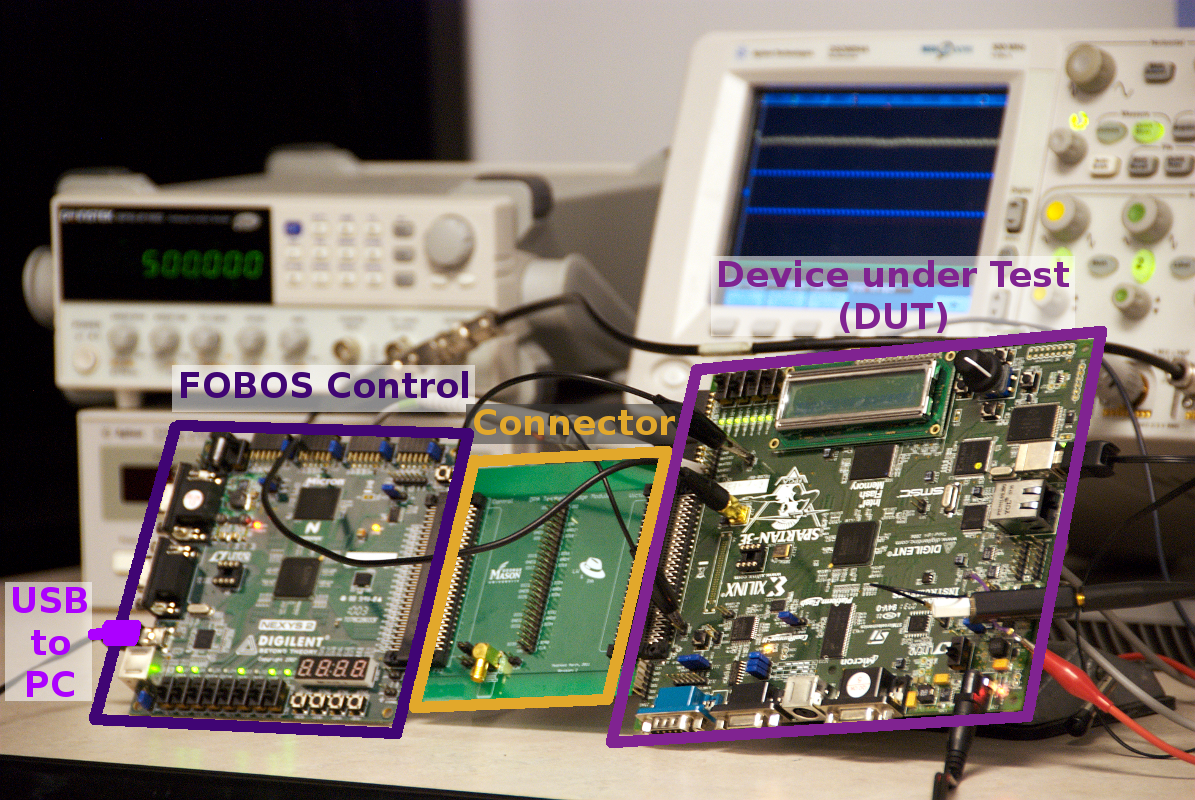
\includegraphics[width=0.9\linewidth]{../figures/FOBOS-label}
        \end{center} 
       \end{block}
     
% ---------------------------------------------------------------------------
      \begin{block}{Acquisition Control}
        \begin{center}
          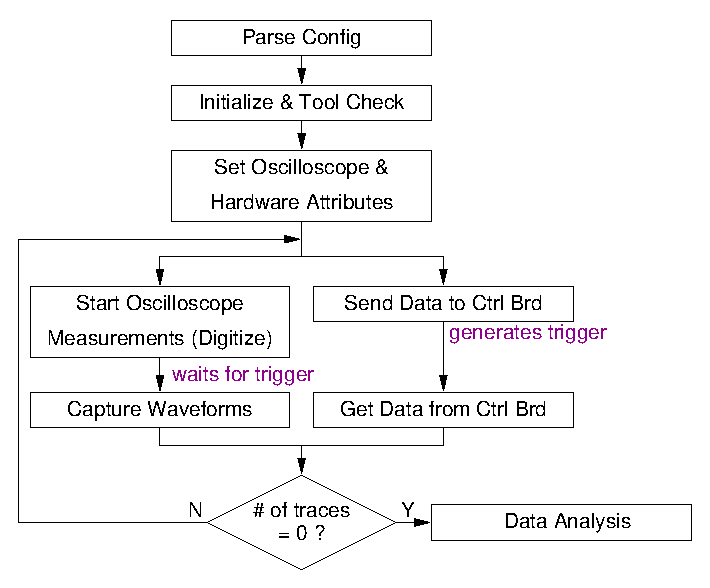
\includegraphics[scale=1.5]{../figures/data_acq}
        \end{center} 
       \end{block}
     
% ---------------------------------------------------------------------------
          
% ---------------------------------------------------------------------------
    \end{column}
% ---------------------------------------------------------------------------
%   THIRD COLUMN
% ---------------------------------------------------------------------------
   \begin{column}{.31\linewidth}
    
% ---------------------------------------------------------------------------
       \begin{block}{FOBOS Analysis}
        \begin{center}
          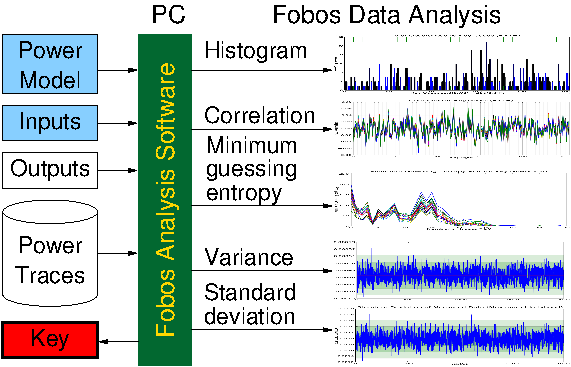
\includegraphics[scale=1.5]{../figures/fobos-dan}
        \end{center} 
       \end{block}
% ---------------------------------------------------------------------------
       \begin{block}{Analysis Workflow}
        \begin{center}
          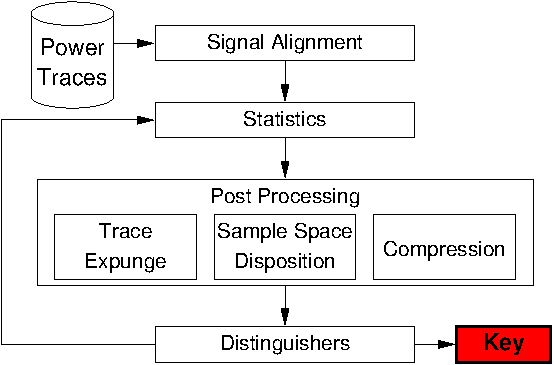
\includegraphics[scale=1.5]{../figures/data_anl}
        \end{center} 
       \end{block}
% ---------------------------------------------------------------------------
       \begin{block}{Signal Alignment}
        \begin{minipage}[t]{0.49\linewidth}
          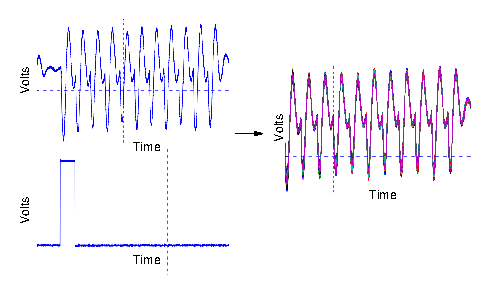
\includegraphics[scale=2.0]{../figures/alignedTraces}
        \end{minipage}%
        \begin{minipage}[t]{0.49\linewidth}
         \begin{itemize}
           \item bla
           \item bla
         \end{itemize} 
        \end{minipage}
       \end{block}
% ---------------------------------------------------------------------------
       \begin{block}{Sample Space Disposition}
        \begin{minipage}[t]{0.49\linewidth}%
          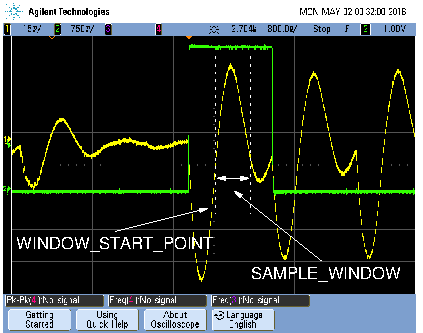
\includegraphics[width=0.9\linewidth]{../figures/oscilloscope-sample-window}
        \end{minipage}%
        \begin{minipage}[t]{0.49\linewidth}%
          \vspace{-6cm}% 
          \begin{itemize}
            \item User can select any part of the trace for further analysis.
            \item Reduces computation time.
          \end{itemize} 
          \begin{center}
            \setbeamercolor{padding}{fg=white, bg=cergbg3}
            \begin{beamercolorbox}[rounded=true]{padding}%
               \footnotesize%
              \begin{lstlisting}
WINDOW_START_POINT = 100
SAMPLE_WINDOW = 1000
              \end{lstlisting}
            \end{beamercolorbox}
          \end{center}
        \end{minipage}
       \end{block}
% ---------------------------------------------------------------------------
       \begin{block}{Compression}
        \begin{minipage}[t]{0.49\linewidth}
		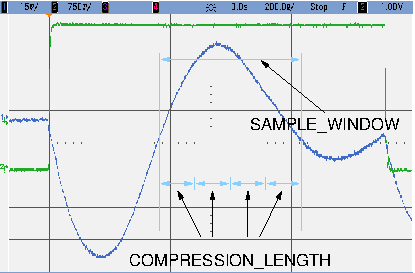
\includegraphics[width=0.9\linewidth]{../figures/oscilloscope-compression-window}
        \end{minipage}%
        \begin{minipage}[t]{0.49\linewidth}%
          \vspace{-6.5cm}% 
         \begin{itemize}
           \item Compress to MAXimum, MINimum, or MEAN of given sample set.
           \item Further reduces number of points for correlation.
         \end{itemize} 
          \begin{center}
            \setbeamercolor{padding}{fg=white, bg=cergbg3}
            \begin{beamercolorbox}[rounded=true]{padding}%
               \footnotesize%
              \begin{lstlisting}
COMPRESSION_LENGTH = 40
COMPRESSION_TYPE = MAX
              \end{lstlisting}
            \end{beamercolorbox}
          \end{center}
        \end{minipage}
       \end{block}
% ---------------------------------------------------------------------------
       \begin{block}{Example: Attack on AES}
         \begin{center}
           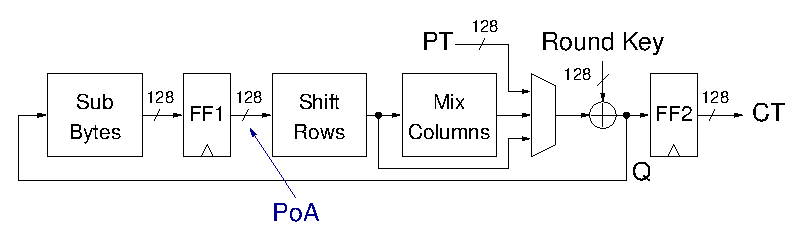
\includegraphics[width=0.9\linewidth]{../figures/aes128}
         \end{center}
         \begin{itemize}
		 \item {\small $PowerGuess_{i, j}$ = HD(SBOX($CT_{i-1}$), SBOX($PT_{i}$ $\oplus$ $KeyGuess_{j}$) )}
		 \item
         \end{itemize}
	 \begin{minipage}[t]{0.49\linewidth}
		 %\begin{center}
			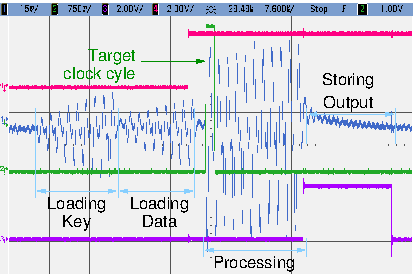
\includegraphics[width=0.80\linewidth]{../figures/oscilloscope-all-4ch} 
		%\end{center}
	 
	 \end{minipage}%
	 \begin{minipage}[t]{0.49\linewidth}  
		 \vspace{-6cm}
		 \begin{itemize}
		  \item 
		  \item 
		 \end{itemize}
         \end{minipage} 
	 
        \begin{minipage}[t]{0.49\linewidth}
           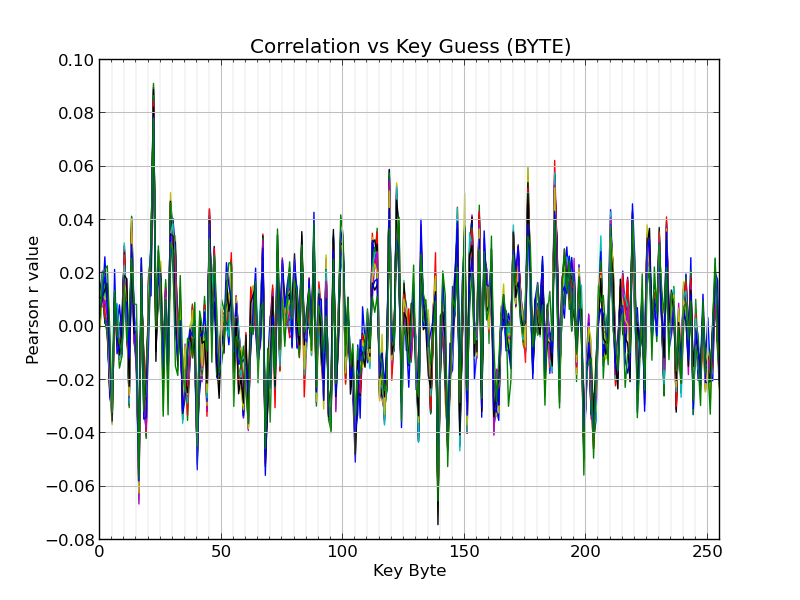
\includegraphics[width=0.9\linewidth]{../figures/pearsonsCoActual}
        \end{minipage}%
        \begin{minipage}[t]{0.49\linewidth}  
		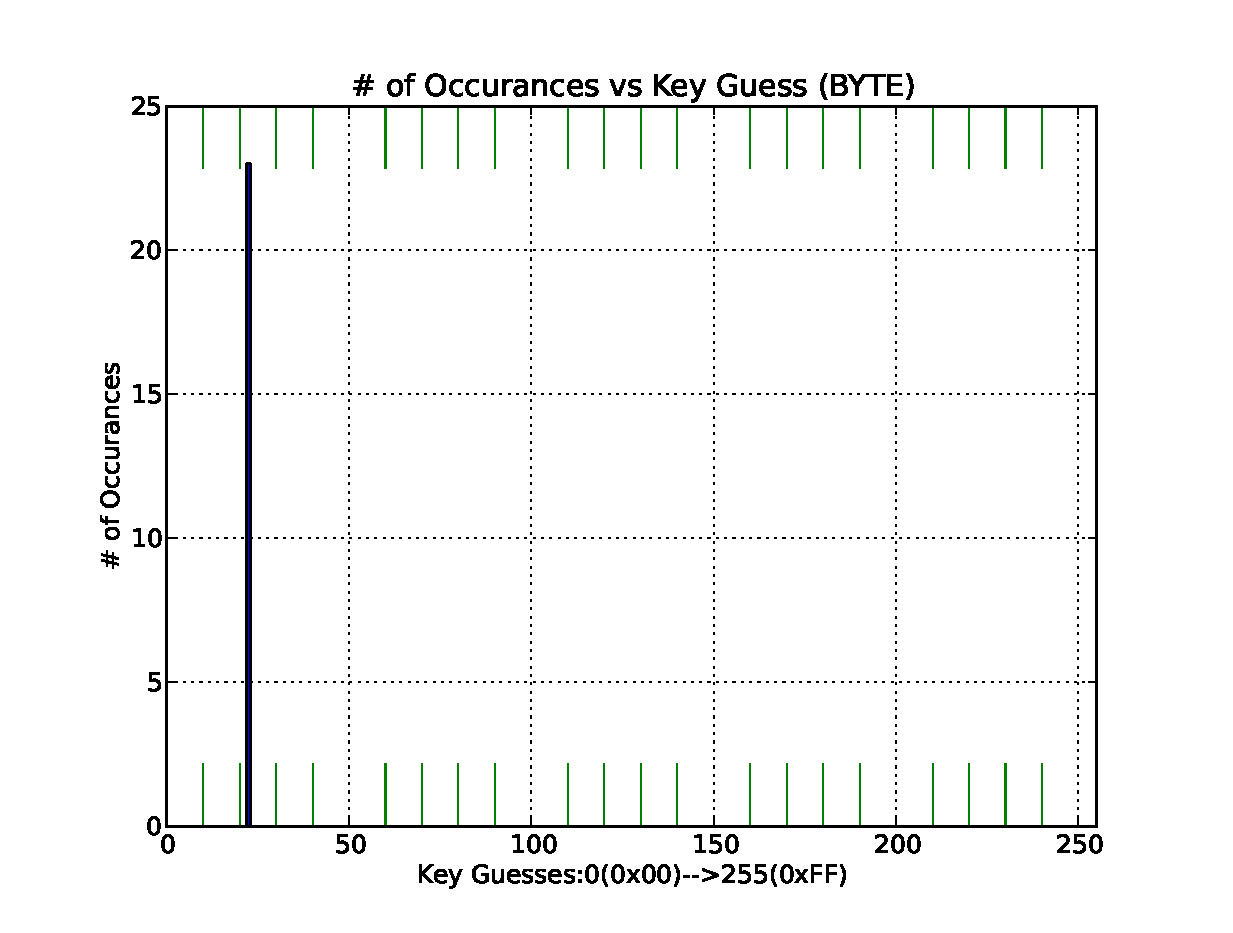
\includegraphics[width=0.9\linewidth]{../figures/histPearsonsCoActual}
        \end{minipage}
	
       \end{block}
% ---------------------------------------------------------------------------
% ---------------------------------------------------------------------------
%      \begin{block}{References}
%        \footnotesize
%          \bibliographystyle{IEEEtran}
%          \bibliography{keccak}
%        %\input{keccakbib}
%      \end{block} 
   \end{column}
\end{columns}

\end{frame}
\end{document}

 
